\ifdefined\ishandout
\documentclass[handout]{beamer}
\else
\documentclass{beamer}
\fi

\usepackage[frenchb]{babel}
\usepackage[T1]{fontenc}
\usepackage[latin1]{inputenc}
\usepackage{hyperref}
\usepackage{multirow}
\usepackage{listings}
\usepackage{fancyvrb}
\usepackage{tikz}
\usepackage{framed}
\usepackage{algorithm}
\usepackage{algorithmic}
\usepackage{xcolor}
\usepackage{color, colortbl}
\usepackage{handoutWithNotes}
\usetikzlibrary{shapes.geometric}
\usetikzlibrary{shapes.arrows, chains}
\usetikzlibrary{arrows}
\usepackage{array}
\usetheme{Boadilla}

\ifdefined\ishandout
\pgfpagesuselayout{3 on 1 with notes}[a4paper,border shrink=5mm]
\usecolortheme{dove}
\else
\usecolortheme{dolphin}
\fi


\lstnewenvironment{codeC}
{ \lstset{language=C,
    otherkeywords={printf,scan}}
}
{}
\newcommand{\red}{\textcolor{red}}
%\newcommand \emph
%Default size : 12.8 cm * 9.6 cm

\ifdefined\ishandout
\newenvironment<>{codeblock}[1]{%begin
  \setbeamercolor{block title}{fg=black,bg=lightgray!80}%
  \begin{block}{#1}}
  % \begin{codeC}}
  %  {\end{codeC}
{  
\end{block}}

\newenvironment<>{termblock}[1]{
    \setbeamercolor{block title}{fg=black,bg=lightgray!90}%
    \begin{block}{#1}}
%     \begin{Verbatim}}
{%\end{Verbatim}
\end{block}
}

\definecolor{bluegreen}{RGB}{0,0,0}
%\definecolor{bluegreen}{rgb}{0,0.6,0.8}
\else

\newenvironment<>{codeblock}[1]{%begin
  \setbeamercolor{block title}{fg=darkgray,bg=yellow}%
  \begin{block}{#1}}
  % \begin{codeC}}
  %  {\end{codeC}
{  
\end{block}}

\newenvironment<>{termblock}[1]{
    \setbeamercolor{block title}{fg=white,bg=lightgray}%
    \begin{block}{#1}}
%     \begin{Verbatim}}
{%\end{Verbatim}
\end{block}
}

\definecolor{bluegreen}{RGB}{0,149,182}
%\definecolor{bluegreen}{rgb}{0,0.6,0.8}
\fi

%\newcommand{\output}[1]{
\setbeamertemplate{navigation symbols}{}
\newcommand{\bvrb}{\Verb[commandchars=���,formatcom=\color{bluegreen}]}



%%% Param�tres du cours (� r�gler)
%Num�ro du cours
\newcommand{\nb}{2}

\title[Cours n�\nb]{Cours n�\nb - Premi�res notions de programmation en langage C}
\author[]{julien.brajard@upmc.fr}
\institute[Polytech' UPMC]{Polytech' UPMC}
\date{5 Octobre 2015}
\begin{document}
%%%%%%%%%%%%%%%%%%%%% SLIDES DE TITRE
\begin{frame}
\titlepage
\centering{
\url{http://australe.upmc.fr} (onglet EPU-C5-IGE Info Gen)}
\end{frame}
%%%%%%%%%%%%%%%%%%%%%
\begin{frame}
\frametitle{Plan du cours n�\nb}
\tableofcontents[hideallsubsections]
\end{frame}

%%%%



%%%%%% SECTION 12
%% !TEX encoding = IsoLatin9

%%%%%%%%%%%%%%%%%%%%% SECTION 1
\section{Le langage C}\label{section:1}
\begin{frame}
  \begin{columns}
    \column{4.8cm}
    \tableofcontents[currentsection,hideothersubsections]
    \column{7cm}
    \centering{
      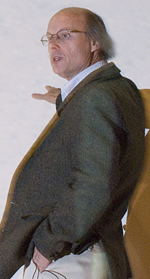
\includegraphics[width=2cm]{fig/stroustrup.jpg}
      
      \textit{``There are only two kinds of programming languages: 
those people always bitch about and those nobody uses.''}\\
      \small{
        \hfill Bjarne Stroustrup, 
        
        \hfill auteur du language de programmation C++.
      }
    }
  \end{columns}
  
\end{frame}

\begin{frame}
\frametitle{Welcome to the machine}
\framesubtitle{Qu'y-a-t'il � l'int�rieur de l'ordinateur ?}
\begin{figure}
\centering
\begin{tikzpicture} [
  label/.style = { 
    rectangle,
    rounded corners,
    text width = 3cm, 
    text badly centered},
  node distance = 5cm
  ]
  \node[inner sep=0pt] (carte) at (0,0)
  {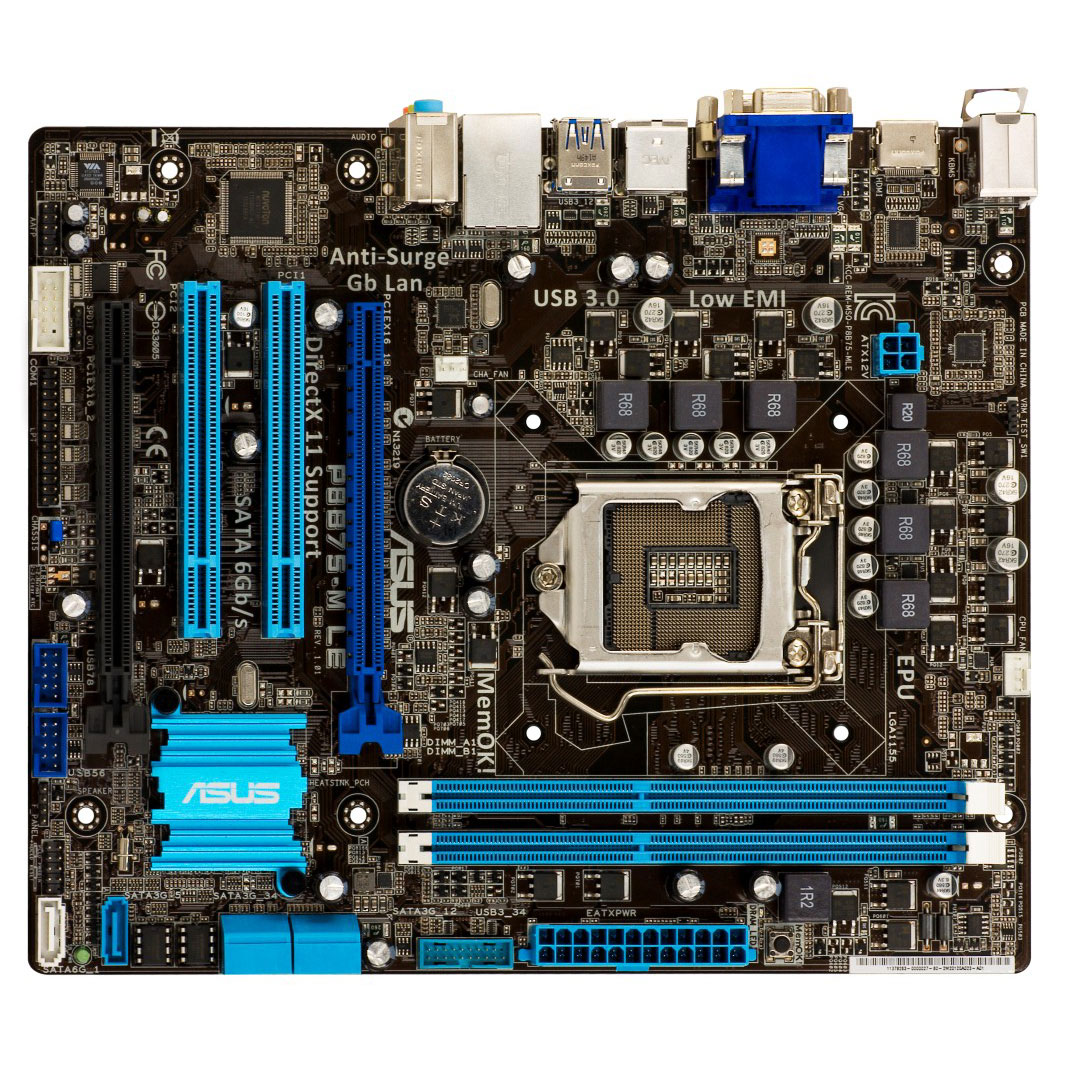
\includegraphics[scale=0.2]{./fig/carte_mere.jpg}};
  \node (mem) [draw, ellipse, very thick, minimum width=4.9cm, minimum height=1cm, color=red] at (1.15,-2) {};
  \node (proc) [draw, ellipse, very thick, minimum width=1.8cm, minimum height=1.8cm, color=orange] at (1,-0.3) {};
  \node (com) [draw, ellipse, very thick, minimum width=4.5cm, minimum height=1.5cm, color=magenta] at (0.8,2.7) {};
  \node (lcom) [label,draw=magenta,right of = com,xshift=+0.2cm] {Des communications avec "l'ext�rieur"};
  \node (lproc)[label,draw=orange,right of = proc] {Une unit� de traitement};
  \node (lmem) [label,draw=red,right of = mem,xshift=-0.15cm] {De la m�moire};

\draw[->,thick,red] (mem) -- (lmem);
\draw[->,thick,orange] (proc) -- (lproc);
\draw[->,thick,magenta] (com) -- (lcom);

\end{tikzpicture}
\end{figure}
\end{frame}

\begin{frame}
\frametitle{Que fait l'ordinateur ?}
\begin{itemize}

\item Un ordinateur traite de fa�on automatique de l'information
\begin{itemize}
\item Sous forme magn�tique ou �lectrique,\\
\item Repr�sentation binaire (i.e. 0 et 1).\\
\end{itemize}

\item Besoin d'abstraction pour repr�sentaiton l'information utilement.
\begin{itemize}
\item Entiers,\\
\item R�els,\\
\item Caract�res,\\
\item Mots.\\
\end{itemize}

\item Besoin d'abstraction pour repr�senter les traitements
\begin{itemize}
\item Affectations,
\item Boucles,
\item Op�ration arithm�tiques,
\item Tests.
\end{itemize}

\end{itemize}

\end{frame}

\begin{frame}
\frametitle{Historique}
\begin{description}
\item[1969 : ] Cr�ation du syst�me UNIX (Lab. Bell, K. Thompson et D. Ritchie). UNIX est intialement �crit en assembleur.\\
\item[1970 : ] K. Thompson d�finit le langage B et r��crit UNIX dans ce langage.\\
\item[1972 : ] D. Ritchie d�finit le langage C.\\
\item[1973 : ] UNIX (version 5) est r��crit en C � 90\%\\
\item[1989 : ] l'ANSI (American National Standard Institute) d�finit une norme du langage C : C ANSI.\\ 
\end{description}
\end{frame}

\begin{frame}
\frametitle{Caract�ristiques du C}
\begin{itemize}
\item Langage de programmation imp�rative.\\
\item Programmation modulaire.\\
\item Langage de bas-niveau (proche du syt�me).\\
\item Simplicit� et minimalit� du langage.\\
\item Biblioth�ques standards assez riches.\\
\item Ex�cutable g�n�r� rapide et de petite taille.\\
\item Langage permissif : faiblement typ� (le compilateur de v�rifie pas tout).\\
\end{itemize}
\end{frame}

\begin{frame}[fragile]
\frametitle{Un programme en C}
\begin{columns}
\column{.5\textwidth}
\begin{figure}
\begin{tikzpicture}[
 block/.style = { 
    rectangle,
    draw=black,
    text width = 3cm, 
    text badly centered},
  node distance = 2cm
  ]
\node(code)[block,fill=yellow]{\verb|Code C|};
\node(exec)[block,fill=lightgray,below of=code]{\verb|Ex�ctuable|};
\draw[->,thick,black] (code) -- (exec);

\end{tikzpicture}
\end{figure}
\column{.5\textwidth}
\begin{itemize}
\item Le \colorbox{yellow}{\texttt{Code C}} est un fichier texte (ASCII) lisible par des �diteurs de texte (emacs, gedit, vi, ...) et donc par vous.\\
\item L'\colorbox{lightgray}{\texttt{Ex�cutable}} est fichier binaire directement interpr�table pas le syt�me (mais illisble par vous).\\
\end{itemize}

\end{columns}
\end{frame}

\begin{frame}[fragile]
\frametitle{Cr�ation d'un programme}
\begin{enumerate}

\item �criture d'un programme dans un �diteur de texte (emacs, gedit, ...)
\begin{itemize}
\item Sauvegarde dans un fichier : \verb|fichier_source.c|
\end{itemize}

\item Compilation sous Linux avec \verb|gcc| (dans un terminal)
\begin{itemize}
\item \verb|gcc -Wall -o fichier_executable fichier_source.c|
\end{itemize}

\item Ex�cution comme une commande (dans un terminal)
\begin{itemize}
\item \Verb[commandchars=\\\{\}]|./fichier_executable\textit{ [param�tres]}|
\end{itemize}

\end{enumerate}
\end{frame}

\begin{frame}[fragile]
\frametitle{Exemple simple : "Hello World"}
\begin{columns}
\column{.5\textwidth}
\begin{itemize}
\item Pr� en-t�te (inclusion de biblioth�ques, ...) commen�ant par \bvrb|#|
\tikz[remember picture,baseline=-.5ex]\coordinate(lbib);
\item Commentaire
\tikz[remember picture,baseline=-.5ex]\coordinate(lcom);
\item D�finition du \bvrb|main| (fonction principale du programme)
\tikz[remember picture,baseline=-.5ex]\coordinate(lmai);
\item Accolade ouvrante \bvrb|{|
\tikz[remember picture,baseline=-.5ex]\coordinate(laco);
\item Bloc d'instruction : suite d'instructions entre \bvrb|{| et \bvrb|}| s�par�es
par des \bvrb|;|
\tikz[remember picture,baseline=-.5ex]\coordinate(lins);
\item Accolade fermante \bvrb|}|
\tikz[remember picture,baseline=-.5ex]\coordinate(lacf);
\end{itemize}
\column{.5\textwidth}
\begin{codeblock}{Fichier hello.c}
\lstset{escapeinside={��}}
\begin{codeC}
�\tikz[remember picture,baseline=-.5ex]\coordinate(bib);�#include <stdio.h>

�\tikz[remember picture,baseline=-.5ex]\coordinate(com);�/* Programme principal */
�\tikz[remember picture,baseline=-.5ex]\coordinate(mai);�int main()
�\tikz[remember picture,baseline=-.5ex]\coordinate(aco);�{
�\tikz[remember picture,baseline=+.5ex]\coordinate(ins);� printf("Hello world");
  return(0);
�\tikz[remember picture,baseline]\coordinate(acf);�}
\end{codeC}
\end{codeblock}
\end{columns}
\begin{tikzpicture}[remember picture,overlay]
\draw (lbib) edge[->, gray,thick] (bib);
\draw (lcom) edge[->, gray,thick] (com);
\draw (lmai) edge[->, gray,thick] (mai);
\draw (laco) edge[->, gray,thick] (aco);
\draw (lins) edge[->, gray,thick] (ins);
\draw (lacf) edge[->, gray,thick] (acf);
\end{tikzpicture}

\begin{alertblock}{}
\centering
En C, une instruction se termine par un point-virgule \red{\textbf{\Large{;}}}
\end{alertblock}

\end{frame}

\begin{frame}[fragile]
\frametitle{Exemple simple : "Hello World"}


\begin{termblock}{Compilation}
\begin{Verbatim}[commandchars=\\\{\}]
\textbf{>>}gcc -Wall hello.c -o hello
\end{Verbatim}
\end{termblock}

\begin{termblock}{Ex�cution}
\begin{Verbatim}[commandchars=\\\{\}]
\textbf{>>}./hello
\end{Verbatim}
\end{termblock}


\begin{termblock}{Le programme affiche � l'�cran}
\begin{Verbatim}[commandchars=\\\{\}]
\textcolor{darkgray}{Hello world}
\end{Verbatim}
\end{termblock}

\end{frame}

\begin{frame}[fragile]
\frametitle{Indentation}
\begin{itemize}
\item La fa�on de pr�senter un programme n'a pas d'impact sur ses performances.\\
\item Mais, indenter un programme le rend plus lisible et donc plus facile � corriger et donc � faire fonctionner.\\
\item Indenter : d�caler de quelques espaces les parties du code dans un bloc.\\
\end{itemize}
\begin{columns}
\column{.47\textwidth}
\begin{codeblock}{Avec indentation}
\lstset{escapeinside={��}}
\begin{codeC}
#include <stdio.h>

/*Programme principal*/
int main()
{
  printf("Hello world");
  return(0);
}
\end{codeC}
\end{codeblock}

\column{.47\textwidth}
\begin{codeblock}{Sans indentation}
\lstset{escapeinside={��}}
\begin{codeC}
#include <stdio.h> /*Pro
gramme principal*/int 
main(){printf("Hello 
world");return(0);}
\end{codeC}
\end{codeblock}

\end{columns}
\end{frame}

%% !TEX encoding = IsoLatin9

%%%%%%%%%%%%%%%%%%%%% SECTION 1
\section{Les commentaires }
\begin{frame}
  \begin{columns}
    \column{4.8cm}
    \tableofcontents[currentsection,hideothersubsections]
    \column{7cm}
    \centering{
      \includegraphics[width=6cm]{fig/code.jpg}
      
      \textit{Eagleson's Law: "Any code of your own that you haven't looked at for six or more months, might as well have been written by someone else."}\\
      \small{
        \hfill Anonyme
      }
    }
  \end{columns}
  
\end{frame}

\begin{frame}[fragile]
\frametitle{Les commentaires}
\begin{itemize}
\item Pour mettre le reste d'une ligne en commentaire, on le pr�c�de de \bvrb|//| :
\begin{codeblock}{}
\lstset{escapeinside={��}}
\begin{codeC}
int a ; // a est un entier
// fin de la d�claraion des variables
\end{codeC}
\end{codeblock}
\item Pour mettre tout un bloc en commentaire, on l'encadre entre \bvrb|/*| et \bvrb|*/| :
\begin{codeblock}{}
\lstset{escapeinside={��}}
\begin{codeC}
#include <stdio.h>

/* Ce qui suit est la fonction principale de hello.c
Elle affiche : hello world*/

int main()
{...
\end{codeC}
\end{codeblock}
\end{itemize}
\end{frame}

\begin{frame}
\frametitle{Remarques sur les commentaires}
\begin{block}{Pourquoi utiliser les commentaires ?}
\begin{itemize}
\item Maintenir le code (le modifier apr�s une semaine, un mois,
un an, ...)\\
\item Travailler en �quipe\\
\item Expliquer une partie d'un algorithme\\
\item Peut permettre le d�boggage (voir cours n$^o$6)\\
\item G�n�rer une documentation automatique (doxygen, javadoc, ...)
\end{itemize}
\end{block}
\begin{alertblock}{Attention}
Commenter un programme fait partie du travail du programmeur (c'est-�-dire : \textbf{vous}).
\end{alertblock}

\end{frame}
%% !TEX encoding = IsoLatin9

%%%%%%%%%%%%%%%%%%%%% SECTION 1
\section{Les variables}
\begin{frame}
  \begin{columns}
    \column{4.8cm}
    \tableofcontents[currentsection,hideothersubsections]
    \column{7cm}
    
  \end{columns}
  
\end{frame}

\begin{frame}
\frametitle{Qu'est-ce qu'une variable ?}
\begin{block}{}
Emplacement destin� � recevoir des donn�es.
\end{block}
\begin{block}{}
Zone situ�e dans la m�moire de l'ordinateur (reper�e par une adresse)
\end{block}
Une variable :
\begin{itemize}
\item peut recevoir une valeur,
\item peut �tre modifi�e,
\item \red{doit} �tre d�clar�e.
\end{itemize}
\end{frame}

\begin{frame}[fragile]
\frametitle{D�claration de variables}
\begin{block}{Syntaxe}
\bvrb| �textit�type_variable nom_variable� ; |
\end{block}
\begin{itemize}
\item Une variable est un "objet" manipul� par le programme,
on peut �galement l'appeler \textit{op�rande}.\\
\item Toute variable doit �tre \red{typ�e}.\\
\item R�gles de nommage d'une variable :
\begin{itemize}
\item Compos�e de lettre, de chiffres et du caract�re \verb|_| uniquement.\\
\item Ne doit pas �tre un mot r�serv� du C.\\
\end{itemize}
\item Le type de la variable doit �tre s�par�e du nom de la variable par un espace.\\
\item Une ligne de d�claration se termine par un \bvrb|;| (comme toute instruction C).\\
\end{itemize}
\end{frame}

\begin{frame}[fragile]
\frametitle{Exemples de d�claration}
\begin{codeblock}{}
\lstset{escapeinside={��}}
\begin{codeC}
float x ;
short n = 10 ;
int j,k;
unsigned int p;
\end{codeC}
\end{codeblock}
\begin{block}{Recommandations}
\begin{itemize}
\item Choisir des noms de variables significatifs
(qui ont un sens) ni trop longs, ni trop courts.\\
\item Attention � bien distinguer majuscules et minuscules.\\
\end{itemize}
\end{block}
\end{frame}

\begin{frame}
\frametitle{Mots r�serv�s en C}
\begin{block}{}
Certains mots sont r�serv�s au langage C, on ne peut les utiliser que
dans un but bien d�fini (impossible de les utiliser pour nommer une variable par exemple).
\end{block}

\begin{table}
\centering
\begin{tabular}{cccc}
        \bvrb|auto|    &     \bvrb|double|    &      \bvrb|int|      &       \bvrb|struct| \\
         \bvrb|break|       &     \bvrb|else|      &      \bvrb|long|     &       \bvrb|switch| \\
         \bvrb|case|        &     \bvrb|enum|      &      \bvrb|register| &       \bvrb|typedef| \\
         \bvrb|char|        &     \bvrb|extern|    &      \bvrb|return|   &       \bvrb|union| \\
         \bvrb|const|       &     \bvrb|float|     &      \bvrb|short|    &       \bvrb|unsigned| \\
         \bvrb|continue|    &     \bvrb|for|       &      \bvrb|signed|   &       \bvrb|void| \\
         \bvrb|default|     &     \bvrb|goto|      &      \bvrb|sizeof|   &       \bvrb|volatile| \\
         \bvrb|do|          &     \bvrb|if|        &      \bvrb|static|   &       \bvrb|while| \\
\end{tabular}
\end{table}
\end{frame}

\begin{frame}[fragile]
\frametitle{Types du langage C}
\begin{table}
\centering
\begin{tabular}{|l|l|l|}
\hline
\bvrb|char| & caract�re & $\geq$8 bits \\
\hline
\bvrb|short| & entier court & $\geq$16 bits \\
\hline
\bvrb|int| & entier & $\geq$16 bits (souvent 32) \\
\hline
\bvrb|long| & entier long & $\geq$32 bits \\
\hline
\bvrb|float| & r�el & 32 bits \\
\hline
\bvrb|double| & r�el double pr�cision & 64 bits \\
\hline
\bvrb|long double| & r�el de longueur max & 128 bits\\
\hline
\end{tabular}
\end{table}

\begin{block}{}
Les donn�es peuvent aussi �tre d�clar�es sign�es (par d�faut)
ou non sign�es(\bvrb|unsigned|).
\end{block}

\textit{Plus de d�tails dans le cours 9.}

\end{frame}


\begin{frame}[fragile]
\frametitle{Quelques utilisations simples}
\begin{itemize}
\item D�claration d'un entier
\begin{codeblock}{}
\lstset{escapeinside={��}}
\begin{codeC}
int n;
\end{codeC}
\end{codeblock}

\item Affectation d'une variable
\begin{codeblock}{}
\lstset{escapeinside={��}}
\begin{codeC}
n = 2;
\end{codeC}
\end{codeblock}
En pseudo-langage, on �crirait : $n \leftarrow 2$.\\

\item Un calcul simple :
\begin{codeblock}{}
\lstset{escapeinside={��}}
\begin{codeC}
int p;
p = 2*n + 1;
\end{codeC}
\end{codeblock}
\end{itemize}
\end{frame}
\begin{frame}[fragile]
\frametitle{Affichage d'une variable}
\begin{codeblock}{}
\lstset{escapeinside={��}}
\begin{codeC}
int n = 2 ;
printf("n est �gal � %d\n",n);
\end{codeC}
\end{codeblock}
\begin{itemize}
\item \bvrb|%d| indique qu'on affiche un entier
\item \bvrb|\n| indique qu'on veut "afficher" un retour � la ligne.
\item \bvrb|,n| affiche le contenu de la variable \verb|n| � la place de \verb|%d|.
\end{itemize}
\begin{termblock}{R�sultat � l'�cran}
\begin{Verbatim}[commandchars=\\\{\}]
\textcolor{darkgray}{n est �gal � 2}
\end{Verbatim}
\end{termblock}

\end{frame}

\begin{frame}[fragile]
\frametitle{Lecture d'une variable}
\begin{codeblock}{}
\lstset{escapeinside={��}}
\begin{codeC}
int n = 2 ;
scanf("%d",&n);
\end{codeC}
\end{codeblock}
\begin{itemize}
\item \bvrb|%d| indique qu'on lit un entier,
\item \bvrb|&n| indique qu'on affecte � la variable \verb|n| la valeur entr�e au clavier.
\end{itemize}
\begin{alertblock}{}
Ne pas oublier le \red{\textbf{\Large \&}}
\end{alertblock}
\textit{Plus de d�tails dans le cours 3.}
\end{frame}
%% !TEX encoding = IsoLatin9

%%%%%%%%%%%%%%%%%%%%% SECTION 1
\section{Op�rateurs}
\begin{frame}
  \begin{columns}
    \column{4.8cm}
    \tableofcontents[currentsection,hideothersubsections]
    \column{7cm}
    
  \end{columns}
  
\end{frame}

\begin{frame}[fragile]
\frametitle{Rappel : l'op�rateur d'affectaction}
\begin{block}{}
L'op�rateur d'affectation est le signe \bvrb|=|
\end{block}
\begin{columns}
\column{0.45\textwidth}
\begin{codeblock}{}
\lstset{escapeinside={��}}
\begin{codeC}
a = 1 ;  �\tikz[remember picture,baseline = -.5ex]\coordinate(a1);�
x = 2 * 3 + 5 ; �\tikz[remember picture,baseline = -.5ex]\coordinate(x);�
a = a + x ; �\tikz[remember picture,baseline = -.5ex]\coordinate(a2);�
\end{codeC}
\end{codeblock}
\column{0.45\textwidth}
\tikz[remember picture,baseline = -.5ex]\coordinate(la1);
\verb|a| re�oit la valeur 1  ;

\tikz[remember picture,baseline = -.5ex]\coordinate(lx);
\verb|x| re�oit la valeur 11 ;

\tikz[remember picture,baseline = -.5ex]\coordinate(la2);
\verb|a| re�oit la valeur 12  ;

\end{columns}
\begin{tikzpicture}[remember picture,overlay]
\draw (la1) edge[->, gray,thick] (a1);
\draw (lx) edge[->, gray,thick] (x);
\draw (la2) edge[->, gray,thick] (a2);
\end{tikzpicture}

\end{frame}

\begin{frame}[fragile]
\frametitle{Les op�rateurs arithm�tiques}
\begin{block}{}
Les expressions arithm�tiques sont �valu�es de 
la gauche vers la droite en prenant compte de 
la pr�s�ance (priorit� des op�rateurs)
\end{block}
\begin {columns}
\column{.4\textwidth}
\begin{table}
\centering
\begin{tabular}{|r|p{3cm}|}
\hline
\bvrb|*| & multiplication \\
\hline
\bvrb|/| & division  \\
\hline
\bvrb|+| & addition \\
\hline
\bvrb|-| & soustraction \\
\hline
\bvrb|-| & reste de la division enti�re (modulo) \\
\hline
\end{tabular}
\end{table}
\column{0.55\textwidth}
\begin{codeblock}{}
\lstset{escapeinside={��}}
\begin{codeC}
a+b*c //  a + (b*c)
-c%d //  (-c)%d
a*b + c%d // (a*b)+(c%d)
-a/-b+c //  ((-a)/(-b))+c
a/b/c //  (a/b)/c
\end{codeC}
\end{codeblock}

\end{columns}
\end{frame}

\begin{frame}[fragile]
\frametitle{Les op�rateurs de comparaison}
\begin{block}{}
Ils permettent de comparer entre elles des expressions ou des variables
\end{block}
\begin{columns}
\column{.55\textwidth}
\begin{table}
\centering
\begin{tabular}{|c|p{4cm}|}
\hline
\bvrb|>| &  strictement sup�rieur �\\
\hline
\bvrb|>=| &   sup�rieur ou �gal �\\
\hline
\bvrb|<| &  strictement inf�rieur �\\
\hline
\bvrb|<=| &  inf�rieur ou �gal �\\
\hline
\bvrb|==| &  �gal �\\
\hline
\bvrb|!=| &  diff�rent de\\
\hline
\end{tabular}
\end{table}

\column{.43\textwidth}
\begin{codeblock}{}
\lstset{escapeinside={��}}
\begin{codeC}
x = 5 ;
y = 4 ;
x > y ; //=1 (vrai)
x == y ; //=0 (faux)
\end{codeC}
\end{codeblock}
\end{columns}

\begin{block}{}
Le r�sultat de la comparaison est un entier de valeur:
\begin{itemize}
\item \bvrb|non nulle| si la comparaison est \red{vraie}.\\
\item \bvrb|0| si la comparaison est \red{fausse}.\\
\end{itemize}
\end{block}

\end{frame}

\begin{frame}[fragile]
\frametitle{Les op�rateurs logiques}
\begin{block}{}
Ils effectuent des op�rations logiques (et, ou, ...) entre
expressions ou variables.
\end{block}
\begin{columns}
\column{0.4\textwidth}
\begin{table}
\centering
\begin{tabular}{|c|p{3cm}|}
\hline
\bvrb|&&| & \textbf{et} logique \\
\hline
\bvrb!||! & \textbf{ou} logique \\
\hline
\bvrb|!| & \textbf{non} logique \\
\hline
\end{tabular}
\end{table}
\column{.55\textwidth}
\begin{table}
\centering
\begin{tabular}{|c|c|c|}
\hline
\verb|x| & 0 (faux) & $\neq$ 0 (vrai) \\
\hline
\verb|!x| & $\neq$ 0 (vrai) & 0 (faux) \\
\hline
\end{tabular}


\end{table}
\end{columns}

%\begin{columns}
%\column{.48\textwidth}
\begin{table}
\centering
\begin{tabular}{|c|c|c|c|}
\hline
\bvrb|x| & \bvrb|y| & \bvrb|(x && y)| & \bvrb!(x ||�y)!\\
\hline
0 (faux) & 0 (faux) & 0 (faux) & 0 (faux) \\
\hline
0 (faux) & $\neq$ 0 (vrai) & 0 (faux) & $\neq$ 0 (vrai)\\
\hline
$\neq$ 0 (vrai) & 0 (faux)  & 0 (faux) & $\neq$ 0 (vrai)\\
\hline
$\neq$ 0 (vrai) & $\neq$ 0 (vrai) & $\neq$ 0 (vrai) & $\neq$ 0 (vrai) \\
\hline
\end{tabular}
\end{table}
%\end{columns}
\end{frame}


\begin{frame}[fragile]
\frametitle{Traitement de bits}
\begin{block}{}
\begin{itemize}
\item Ils permettent des manipulations au niveau des bits
dans la repr�sentation binaire des nombres\\
\item On ne peut les appliquer que sur des op�randes entiers
(\bvrb|short|, \bvrb|int|, \bvrb|long|), sign� ou non.\\
\end{itemize}
\end{block}
\begin{columns}
\column{.43\textwidth}
\begin{table}
\centering
\begin{tabular}{|c|p{4cm}|}
\hline
\bvrb|&| &  ET bit � bit\\
\hline
\bvrb!|! &   OU inclusif bit � bit\\
\hline
\bvrb|^| &  OU exclusif bit � bit\\
\hline
\bvrb|<<| &  d�calage � gauche\\
\hline
\bvrb|>>| &  d�calage � droite\\
\hline
\bvrb|~| &  compl�ment � un\\
\hline
\end{tabular}
\end{table}

\column{.55\textwidth}
\begin{codeblock}{}
\lstset{escapeinside={��}}
\begin{codeC}
int a = 5;// a=0101(binaire)
int b = 12;//b=1100(binaire)
int c ;
c = a & b ; // c = ...
c = a | b ; // c = ...
c = a ^ b ; // c = ...
c = a << 1 ; // c = ...
c = b >> 1 ; // c = ...
c = ~b ; // c = -13 
\end{codeC}
\end{codeblock}

\end{columns}
\end{frame}


\begin{frame}[fragile]
\frametitle{Incr�mentation/D�cr�mentation}
\begin{block}{}
Incr�menter(\bvrb|++|) ou d�cr�menter (\bvrb|--|) de 1 une variable.
\end{block}
\begin{codeblock}{}
\lstset{escapeinside={��}}
\begin{codeC}
x++ ; // x = x+1
--y ; // y = y-1
\end{codeC}
\end{codeblock}

\begin{itemize}
\item Si l'op�rateur est plac� avant la variable (pr�fix�), celle-ci est incr�ment�e (ou d�cr�ment�e) avant son utilisation.\\
\item Si l'op�rateur est plac� apr�s la variable (postfix�), cell-ci est incr�ment�e (ou d�cr�ment�e) apr�s son utilisation.\\
\end{itemize}
\begin{columns}

\column{0.48\textwidth}
\begin{codeblock}{}
\lstset{escapeinside={��}}
\begin{codeC}
a = 2 ;
b = a++ ;// b=2, a=3
\end{codeC}
\end{codeblock}

\column{0.48\textwidth}
\begin{codeblock}{}
\lstset{escapeinside={��}}
\begin{codeC}
a = 2 ;
b = ++a ;// a=3, b=3
\end{codeC}
\end{codeblock}

\end{columns}
\begin{alertblock}{}
Utilisez l'op�rateur seul pour �viter les erreurs.
\end{alertblock}

\end{frame}

\begin{frame}[fragile]
\frametitle{Op�rateurs d'affectation �largie}
\begin{block}{}
Ils permettent d'all�ger l'�criture des op�rations de mise � jour de variable.
\end{block}
\begin{codeblock}{}
\lstset{escapeinside={��}}
\begin{codeC}
x += b ; // x = x + b
x -= b ; // x = x - b
x /= b ; // x = x / b
x *= b ; // x = x * b
x %= b ; // x = x % b
x |= b ; // x = x | b
x &= b ; // x = x & b
x <<= b ; // x = x << b
x >>= b ; // x = x >> b
\end{codeC}
\end{codeblock}
\begin{alertblock}{}
Attention de ne pas confondre avec l'op�rateur de comparaison
\bvrb|<=|.
\end{alertblock}
\end{frame}

\begin{frame}[fragile]
\frametitle{L'op�rateur conditionnel}
\centering 
\bvrb|�textit�expr1� ? �textit�expr2�  : �textit�expr3� |
\begin{block}{}
Cet op�rateur (ternaire) permet d'agir en fonction du r�sultat
d'�valuation d'une expression.
\end{block}
On �value \bvrb|�textit�expr1�| :
\begin{itemize}
\item Si elle est vraie (donc non nulle), on �value \bvrb|�textit�expr2�|\\
\item Sinon, on �value \bvrb|�textit�expr3�|
\end{itemize}

\begin{codeblock}{}
\lstset{escapeinside={��}}
\begin{codeC}
int x = 5, y = 4, z ;
z = (x>y) ? x : y ;
\end{codeC}
\end{codeblock}
Si \verb|x>y|, \verb|z| prend la valeur de \verb|x|, 
sinon celle de \verb|y|. 
\end{frame}

\begin{frame}[fragile]
\frametitle{R�capitulatif : les op�rateurs du C}
\begin{columns}
\column{0.65\textwidth}
\begin{table}
\centering
\begin{tabular}{|r|l|}
\hline
Unaires & \bvrb|() [] -> .| \\
\hline
Unaires & \bvrb|! + - ++ -- * & sizeof()| \\
\hline
Arithm�tiques & \bvrb|* / %| \\
\hline
D�calages & \bvrb|<< >>| \\
\hline
Comparaison & \bvrb|< <= > >=| \\
\hline
Egalit�s & \bvrb|== !=|\\
\hline
Manip. bits & \bvrb|&| \\
\hline
Manip. bits & \bvrb|^| \\
\hline
Manip. bits & \bvrb!|! \\
\hline
Logiques & \bvrb|&&| \\
\hline
Logiques & \bvrb!||! \\
\hline
Conditionnel & \bvrb|? :|\\
\hline
Affectations & \bvrb!= += *= ^= %= &= |= <<= >>=! \\
\hline
\end{tabular}
\end{table}
\column{0.33\textwidth}
\begin{itemize}
\item Les op�rateurs sur une m�me ligne ont m�me priorit�.\\
\item Les lignes sont class�es dans l'ordre d�croissant de priorit�.\\
\end{itemize}
\end{columns}
\end{frame}


% !TEX encoding = IsoLatin9

%%%%%%%%%%%%%%%%%%%%% SECTION 1
\section{Structures de contr�le et r�p�titive}
\begin{frame}
  \begin{columns}
    \column{4.8cm}
    \tableofcontents[currentsection,hideothersubsections]
    \column{7cm}
    
  \end{columns}
  
\end{frame}

\begin{frame}[fragile]
\frametitle{Introduction}
\begin{block}{Pour un comportement "intelligent" du programme}
\begin{itemize}
\item Possibilit� d'effectuer des \red{choix}, de se comporter
diff�remment suivant les "circonstances" (\red{test}):

Instructions \bvrb|if...else| et \bvrb|switch|\\
\item Possibilit� de \red{r�p�ter plusieurs fois} un ensemble 
d'instructions (\red{boucle}) :

Instructions \bvrb|do...while|, \bvrb|while| et \bvrb|for|\\
\end{itemize}
\end{block}
\end{frame}

\begin{frame}[fragile]
\frametitle{L'instruction \bvrb|if...else|}
\begin{block}{}
Permet d'exprimer une prise de d�cision entre \red{2 choix}.
\end{block}
\begin{columns}
\column{.42\textwidth}
\begin{block}{}
\bvrb|if (�textit�expression�)|\\
\bvrb|   �textit�bloc_instructions1;�|\\
\end{block}
\begin{block}{}
\bvrb|if (�textit�expression�)|\\
\bvrb|   �textit�bloc_instructions1;�|\\
\bvrb|else|\\
\bvrb|   �textit�bloc_instructions2;�|\\
\end{block}
\column{.55\textwidth}
\begin{itemize}
\item \bvrb|�textit�expression�| : expression � �valuer (vraie ou fausse)\\
\item \bvrb|�textit�bloc_instructions1�| : bloc d'instructions, ou instruction simple
� effectuer si \bvrb|�textit�expression�| est \red{vraie}.\\
\item \bvrb|�textit�bloc_instructions2�| : bloc d'instructions, ou instruction simple
� effectuer si \bvrb|�textit�expression�| est \red{fausse}.
Ce bloc est optionnel.\\

\end{itemize}
\end{columns}
\begin{block}{}
Possibilit� d'imbriquer des instructions \bvrb|if..else| dans d'autres expressions \bvrb|if..else|.
Le \bvrb|else| se rapporte au dernier \bvrb|if| rencontr�.
\end{block}
\end{frame}


\begin{frame}[fragile]
\frametitle{L'instruction \bvrb|if...else|}
\framesubtitle{Exemple}
\begin{exampleblock}{}
\begin{algorithmic}[0]
\IF{somme introduite = prix de la boisson}
\STATE Delivrer boisson
\STATE nbre\_boissons $\leftarrow$  nbre\_boissons - 1
\ENDIF
\end{algorithmic}
\end{exampleblock}

\begin{codeblock}{}
\lstset{escapeinside={��}}
\lstset{basicstyle=\scriptsize}
\begin{codeC}
#include <stdio.h>

int main()
{
...
float somme = 0 ;
...
if (somme == prix_boisson)
    {
    printf("Voici votre boisson\n");
    nb_boissons--;
    }
...
}
\end{codeC}
\end{codeblock}


\end{frame}

\begin{frame}[fragile]
\frametitle{L'instruction \bvrb|if...else|}
\framesubtitle{Exemple}
\begin{columns}
\column{.48\textwidth}
\begin{codeblock}{Max de 2 entiers}
\lstset{escapeinside={��}}
\lstset{basicstyle=\scriptsize}
\begin{codeC}
#include <stdio.h>

int main()
{
  int max, a, b;
  printf("Entrez 2 nombres :");
  scanf("%d %d",&a,&b);
  if (a > b) {
    max = a ;
    b = 0;    
  }
  else {
    max = b ;
    a = 0 ;
     }
  printf("maximum : %d\n",max);
}
\end{codeC}
\end{codeblock}
\column{.48\textwidth}
\begin{codeblock}{valeur absolue}
\lstset{escapeinside={��}}
\lstset{basicstyle=\scriptsize}
\begin{codeC}
#include <stdio.h>

int main()
{
  int val_abs, n;
  printf("Entrez 1 nombre :");
  scanf("%d",&n);
  if (n > 0) {
    val_abs = n ;
    }
  else {
    val_abs = -n ;
    }
  printf("v. a. de %d : %d\n",
      n,val_abs);
}
\end{codeC}
\end{codeblock}

\end{columns}
\end{frame}

\begin{frame}[fragile]
\frametitle{L'instruction \bvrb|switch|}
\begin{block}{}
Permet d'exprimer une prise de d�cision � \red{choix multiple}.
\end{block}
\begin{columns}
\column{.45\textwidth}
\begin{block}{}
\bvrb|switch (�textit�expression�) {|\\
\bvrb|   case �textit�constante_1�:|\\
\bvrb|      �textit�bloc_instructions1�|\\
\bvrb|   ......|\\
\bvrb|   case �textit�constante_N�:|\\
\bvrb|      �textit�bloc_instructionsN�|\\
\bvrb|   default:|\\
\bvrb|      �textit�bloc_instructions�|\\
\bvrb|}|
\end{block}
\column{.55\textwidth}
\begin{itemize}
\item Les arguments des \bvrb|case| et \bvrb|�textit�expression�| doivent �tre des
\red{entiers}.\\
\item Si la valeur de  \bvrb|�textit�expression�| correspond � l'un des arguments
de \bvrb|case|, alors le bloc d'instruction correspond est ex�cut�\\
\item L'alternative \bvrb|default| est optionnelle\\

\end{itemize}
\end{columns}
\begin{alertblock}{}
\red{Attention}, � partir du moment o� on est entr� dans un \bvrb|case|,
on execute toutes les instructions des \bvrb|case| au-dessous jusqu'� rencontrer un 
\bvrb|break| qui nous fait sortir du \bvrb|switch|.
\end{alertblock}
\end{frame}

\begin{frame}[fragile]
\frametitle{L'instruction \bvrb|switch|}
\framesubtitle{exemple 1}

\begin{codeblock}{d�termination du prix d'une boisson}
\lstset{escapeinside={��}}
\lstset{basicstyle=\scriptsize}
\begin{codeC}
...
int selection ;
...
switch (selection)
{
  case 0 : prix_boisson = prix_jus_orange ;
           break ;
  case 1 : prix_boisson = prix_eau_plate ;
           break ;
  case 2 : prix_boisson = prix_eau_gazeuse ;
           break ;
  default : printf("Erreur de selection\n");
}  
...
\end{codeC}
\end{codeblock}

\end{frame}

\begin{frame}[fragile]
\frametitle{L'instruction \bvrb|switch|}
\framesubtitle{exemple 2}

\begin{columns}
\column{.48\textwidth}

\begin{codeblock}{}
\lstset{escapeinside={��}}
\lstset{basicstyle=\scriptsize}
\begin{codeC}
#include <stdio.h>

int main()
{
 int a ;
 printf("\nEntrez un nombre :");
 scanf("%d",&a);
 switch (a)
 {
  case 0 : printf("\nNul");
           break;
  case 1 :
  case 2 : printf("\nPetit");
  case 3 :
  case 4 : printf("\nMoyen");
           break;
  default : printf("\Grand");
 }
}
\end{codeC}
\end{codeblock}

\column{0.48\textwidth}
\begin{termblock}{Test d'ex�cution}
\lstset{escapeinside={��}}
\begin{lstlisting}
�\color{darkgray}{\texttt{  Entrez un nombre :}}�1
�\color{darkgray}{\texttt{  Petit}}�
�\color{darkgray}{\texttt{  Moyen}}�

�\color{darkgray}{\texttt{  Entrez un nombre :}}�3
�\color{darkgray}{\texttt{  Moyen}}�

�\color{darkgray}{\texttt{  Entrez un nombre :}}�852
�\color{darkgray}{\texttt{  Grand}}�

�\color{darkgray}{\texttt{  Entrez un nombre :}}�-1
�\color{darkgray}{\texttt{  Grand}}�
\end{lstlisting}
\end{termblock}

\end{columns}

\end{frame}

\begin{frame}[fragile]
\frametitle{La boucle \bvrb|for|}
\begin{block}{}
Permet de r�p�ter une m�me action un
\red{certain nombre de fois} (g�n�ralement connu � l'avance).
\end{block}

\begin{block}{}
\bvrb |for ( �textit�expr1� ; �textit�expr2� ; �textit�expr3� )|\\
\bvrb |  �textit�bloc_instructions�|
\end{block}

\begin{itemize}

\item \bvrb|�textit�expr1�| : condition initiale fix�e.\\
\item \bvrb|�textit�expr2�| : Test de continuation de boucle. Le \bvrb|�textit�bloc_instructions�|
est ex�cut� tant que cette valeur est vraie (et s'arr�te quand elle est fausse).\\
\item \bvrb|�textit�expr3�| : Op�ration effectu�e � chaque tour de boucle (ex : incr�mentation).\\
\end{itemize}

Toutes ces expressions sont facultatives. \bvrb|for (;;)| est une boucle infinie.

\end{frame}

\begin{frame}[fragile]
\frametitle{La boucle \bvrb|for|}
\framesubtitle{Exemple}
\begin{columns}
\column{.48\textwidth}
\begin{codeblock}{}
\lstset{escapeinside={��}}
\lstset{basicstyle=\scriptsize}
\begin{codeC}
#include <stdio.h>

int main()
{
 int i;
 for (i=1 ; i <= 5 ; i++)
 {
  printf("\nBonjour %d fois",i);
 }
}
\end{codeC}
\end{codeblock}

\column{.48\textwidth}
\begin{termblock}{Test d'ex�cution}
\lstset{escapeinside={��}}
\begin{lstlisting}
�\color{darkgray}{\texttt{  Bonjour 1 fois}}�
�\color{darkgray}{\texttt{  Bonjour 2 fois}}�
�\color{darkgray}{\texttt{  Bonjour 3 fois}}�
�\color{darkgray}{\texttt{  Bonjour 4 fois}}�
�\color{darkgray}{\texttt{  Bonjour 5 fois}}�
\end{lstlisting}
\end{termblock}

\end{columns}
Ne pas oublier de \red{d�clarer} la variable de boucle \verb|i|.
\begin{itemize}
\item \Verb|i=1| : On entre dans la boucle avec \verb|i| initialis� � \verb|1|.\\
\item \Verb|i<=5| : On repasse dans la boucle tant que i reste inf�rieur ou �gal � \verb|5|.\\
\item \Verb|i++| : A chaque passage dans la boucle, \verb|i| est incr�ment� de \verb|1|.\\
\item A chaque passage dans la boucle, on affiche \verb|Bonjour| puis la valeur de \verb|i| puis le mot \verb|fois|.
\end{itemize}

\end{frame}


\begin{frame}[fragile]
\frametitle{La boucle \bvrb|while|}
\begin{block}{}
Permet de r�p�ter une m�me action
\red{tant qu'une condition est vraie} (g�n�ralement conna�t pas � l'avance
le nombre d'it�ration effectu�es par la boucle).
\end{block}

\begin{block}{}
\bvrb |while ( �textit�condition� )|\\
\bvrb |  �textit�bloc_instructions�|
\end{block}

\begin{itemize}

\item \bvrb|�textit�condition�| est �valu�e, puis, si elle est vraie \bvrb |�textit�bloc_instructions�| s'ex�cute, puis
on r��value \bvrb|�textit�condition�|,  si elle est vraie \bvrb |�textit�bloc_instructions�| s'ex�cute, etc.\\
\item \bvrb|�textit�condition�| est donc �valu�e avant chaque passage dans le corps de la boucle. \red{On n'est pas s�r d'ex�cuter au moins une fois le bloc d'instructions.}\\
\item Si des variables doivent changer de valeur � chaque passage de boucle, il est n�cessaire des les mettre � jour dans  \bvrb |�textit�bloc_instructions�|.
\end{itemize}

\end{frame}

\begin{frame}[fragile]
\frametitle{La boucle \bvrb|while|}
\framesubtitle{Exemple}


\begin{codeblock}{}
\lstset{escapeinside={��}}
%\lstset{basicstyle=\scriptsize}
\begin{codeC}
...
while(nb_boissons != 0)
{
 printf("Voulez-vous prendre une boissons ? ") ;
 scanf("%d",&choix);
 if (choix==1)
 //Le code 1 correspond � la r�ponse "oui"
 {
  nb_boissons--;
 }
}
\end{codeC}
\end{codeblock}


\end{frame}


\begin{frame}[fragile]
\frametitle{La boucle \bvrb|do...while|}
\begin{block}{}
Permet de r�p�ter une m�me action
\red{tant qu'une condition est vraie} (g�n�ralement conna�t pas � l'avance
le nombre d'it�ration effectu�es par la boucle).
\end{block}

\begin{block}{}
\bvrb |do|\\
\bvrb |{|\\
\bvrb |  �textit�bloc_instructions�|\\
\bvrb |} while ( �textit�condition� )|\\
\end{block}

\begin{itemize}

\item \bvrb |�textit�bloc_instructions�| s'ex�cute, puis \bvrb|�textit�condition�| est �valu�e, puis, si elle est vraie \bvrb |�textit�bloc_instructions�| s'ex�cute, puis
on r��value \bvrb|�textit�condition�|, etc.\\
\item \bvrb|�textit�condition�| est donc �valu�e apr�s chaque passage dans le corps de la boucle. \red{On est s�r d'ex�cuter au moins une fois le bloc d'instructions.}\\
\item Si des variables doivent changer de valeur � chaque passage de boucle, il est n�cessaire des les mettre � jour dans  \bvrb |�textit�bloc_instructions�|.
\end{itemize}

\end{frame}


\begin{frame}[fragile]
\frametitle{La boucle \bvrb|do...while|}
\framesubtitle{2 exemples}
\begin{columns}
\column{0.6\textwidth}
\begin{codeblock}{}
\lstset{escapeinside={��}}
\lstset{basicstyle=\scriptsize}
\begin{codeC}
int main()
{
 int i=1, x=20;
 do
 {
  i = i*2 ;
 } while (i<x);
}
\end{codeC}
\end{codeblock}
\column{0.35\textwidth}
\begin{block}{A la fin de l'ex�cution}
\begin{itemize}
\item \verb|i =|
\ifdefined\correction \only<1>{\Verb|...|}\only<2->{32}
\else                 \only<1->{\Verb|...|}
\fi
\item \verb|x =|
\ifdefined\correction \only<1>{\Verb|...|}\only<2->{20}
\else                 \only<1->{\Verb|...|}
\fi

\end{itemize}
\end{block}
\end{columns}

\ifdefined\correction \pause[3]
\else \pause[2]
\fi

\begin{columns}
\column{0.6\textwidth}
\begin{codeblock}{}
\lstset{escapeinside={��}}
\lstset{basicstyle=\scriptsize}
\begin{codeC}
int main()
{
 int i=1, x=20;
 do
 {
  i = i*2 ;
  x = x/2 ;
 } while ( (i<x) && (x>0) );
}
\end{codeC}
\end{codeblock}
\column{0.35\textwidth}
\begin{block}{A la fin de l'ex�cution}
\begin{itemize}
\item \verb|i =|
\ifdefined\correction \only<3>{\Verb|...|}\only<4->{8}
\else                 \only<2->{\Verb|...|}
\fi
\item \verb|x =|
\ifdefined\correction \only<3>{\Verb|...|}\only<4->{2}
\else                 \only<2->{\Verb|...|}
\fi


\end{itemize}
\end{block}
\end{columns}

\end{frame}

\begin{frame}[fragile]
\frametitle{Quel type de boucle choisir ?}
\begin{figure}
\centering
\begin{tikzpicture} [
    auto,
    block/.style    = { rectangle, draw=blue, thick, 
                        text width=7cm, text centered,
                        rounded corners, minimum height=2em },
    line/.style     = { draw, thick, ->, shorten >=2pt },
    node distance=3cm,
  ]
  \node (rac) [block] {Est-ce que je connais � l'avance le nombre d'it�rations ?};
  \node (fils1)[below of = rac]{};
  \node (for) [left of = fils1] {boucle \bvrb|for|};
  \node (right) [block, right of = fils1] 
  {Est-ce que je veux effectuer au moins une fois les instructions avant de tester la condition d'arr�t ?};
  \node (fils2) [below of = right]{};
  \node (do) [left of = fils2] {boucle \bvrb|do...while|};
  \node (while) [right of = fils2] {boucle \bvrb|while|};

  
  % connect nodes
  \begin{scope}[every path/.style=line]
  \path (rac) -- node [midway, left]{oui} (for);
  \path (rac) -- node [midway, right]{non} (right);
  \path (right) -- node [midway, left]{oui} (do);
  \path (right) -- node [midway, right]{non} (while);

  \end{scope}

\end{tikzpicture}
\end{figure}
\end{frame}
\end{document}

%%%%%%%%%%%%%%%%%%%%% SECTION 1
\section{Les algorithmes}\label{section:1}
\begin{frame}
\begin{columns}
        \column{4.8cm}
            \tableofcontents[currentsection]
        \column{7cm}
        \centering{
            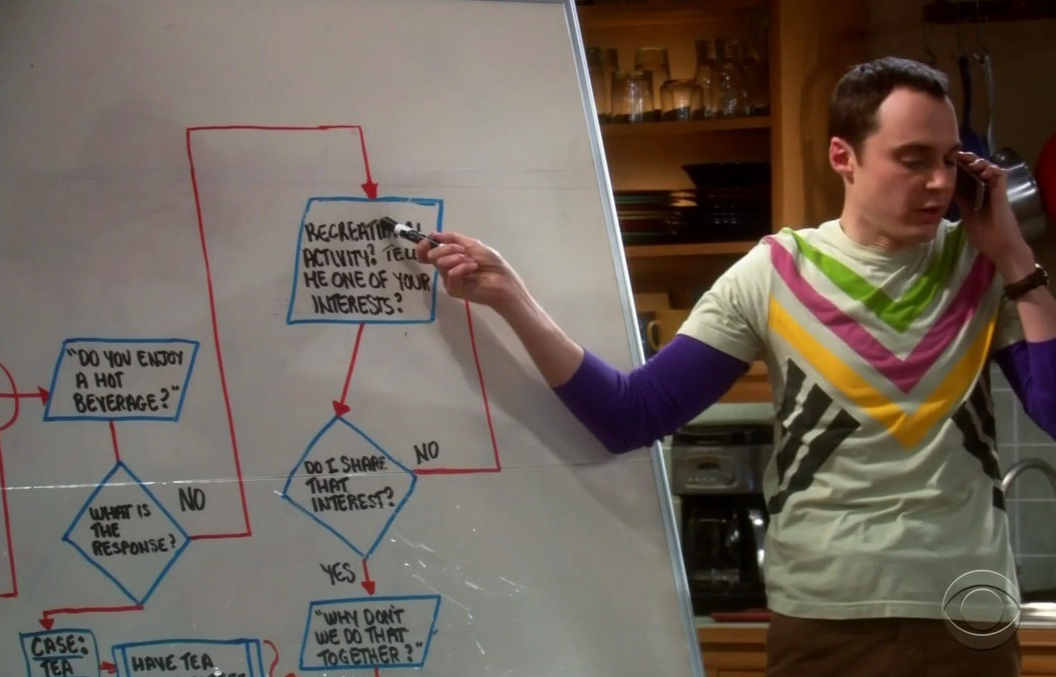
\includegraphics[width=7cm]{fig/Algorithm-sheldon.png}
            
                 \textit{ I believe I've isolateblblblblblblsblbslbslbsl
            sblbslblsblsblblsblbs
            lbslblbslsb d the algorithm for making friends.}
     
            
            \small{
            \hfill Sheldon Cooper, 
            
            \hfill in \textit{The Big Band Theory}, Season 2, Episode 13
            }
}

    \end{columns}

\end{frame}


%%%%%%%%%%%%%%%%%%%%%
\subsection{Introduction}
    \begin{frame}
    \frametitle{Pourquoi faire appel � des algorithmes ?}
    Pour automatiser des t�ches
    
    Exemples :
    \begin{itemize}
    \item M�tier � tisser\\
    \item M�thode de calcul � la main d'une division\\
    \item Recette de cuisine\\
    \item ...\\
    \end{itemize}
    \end{frame}
 
 %%%%%%%%%%%%%%%%%
 
    \begin{frame}
    \frametitle{Qu'est-ce qu'un algorithme ?}
    \begin{block}{D�finition}
    Un algorithme est un ensemble 
    ordonn� d'instructions simples
permettant de r�soudre un probl�me.
    \end{block}
    \end{frame}
    
 %%%%%%%%%%%%%%%%%%
 \subsection{Construction d'un algorithme}
%%%%%%%%%%%%%%%%%%%    
\section{La machine de Turing}
%%%%%%%%%%%%%%%%%%%%
 
  
\begin{frame}[fragile]
\frametitle{Un peu d'histoire...}
\begin{codeblock}{Test}
\begin{codeC}
for (int i = 0 ; i < n ; i ++) {
    //a comment
    printf("%d",i);
    }
\end{codeC}
\end{codeblock}

\begin{termblock}{test 2}
\lstset{escapeinside={��}}
\begin{lstlisting}
�\textbf{>>}�./a.out
�\color{darkgray}{\texttt{  Hello World}}�
\end{lstlisting}
\end{termblock}

 \begin{block}{Bloc standard}
blablabla
\end{block}
\end{frame}


\begin{frame}[fragile]
\frametitle{essai}
\begin{columns}
\column{6cm}
\begin{block}

\begin{figure}
\begin{tikzpicture} [
    auto,
    decision/.style = { diamond, draw=blue, thick, fill=blue!20,
                        text width=5em, text badly centered,
                        inner sep=1pt, rounded corners },
    block/.style    = { rectangle, draw=blue, thick, 
                        fill=blue!20, text width=10em, text centered,
                        rounded corners, minimum height=2em },
    line/.style     = { draw, thick, ->, shorten >=2pt },
  ]
   \matrix [column sep=-10mm, row sep=10mm] {
                    & \node [text centered] (x) {$\mathbf{X}$};            & \\
                    & \node (null1) {};                                    & \\
                    & \node [block] (doa) {\textsf{DoAE}($\mathbf{X}$)};   & \\
  	               \node(null3){}; & \node [decision] (uiddes)
                        {\textsf{UID}($\hat{\mathbf{X}}$)};
                                  & \node[text centered](tra){$\mathbf{i}$}; \\
                  & \node [block] (track) {\textsf{DoAT}($\mathbf{x}$)}; & \\
                    & \node [block] (pesos)
                        {\textsf{BF}(DoA$_{\mathrm{T}}$,DoAs)};            & \\
                    & \node [block] (filtrado)
                        {\textsf{SF}($\mathbf{w}$,$\mathbf{x}$)};          & \\
                    & \node [text centered] (xf) {$\hat{x}(t)$ };          & \\
  };
  % connect all nodes defined above
 \begin{scope} [every path/.style=line]
    \path (x)        --    (doa);
    \path (doa)      --    node [near start] {DoAs} (uiddes);
    \path (tra)      --    (uiddes);
    \path (uiddes)   --++  (-3,0) node [near start] {no} |- (null1);
    \path (uiddes)   --    node [near start] {DoA} (track);
    \path (track)    --    node [near start] {DoA$_{\mathrm{T}}$} (pesos);
    \path (pesos)    --    node [near start] {\textbf{w}} (filtrado);
    \path (filtrado) --    (xf);
  
  \end{scope}
\end{tikzpicture}
\end{figure}
\end{block}
\column{3cm}
\begin{block}{bulbul}
\end{block}
\end{columns}
\end{frame}

\end{document}
